 \section{Implementierung der Mitarbeiteransicht}

Alle relevanten Codeteile, sowie zusätzliche Dokumentationen sind im GitHub Repository verfügbar, das unter dem folgenden Verweis zugänglich ist: \textit{\cite{equilibriaSharingFrontend}}. In diesem Repository finden sich sowohl
die Quellcodes für die Implementierung als auch ergänzende Dateien, die zur Dokumentation und zum besseren Verständnis des Projekts beitragen.

\subsection{Struktur}
Die folgende Diagrammbeschreibung [\ref{fig:navigationsfluss}] zeigt den grundlegenden Aufbau der Equilibria Sharing-Mitarbeiteransicht:

\begin{figure}
	\centering
	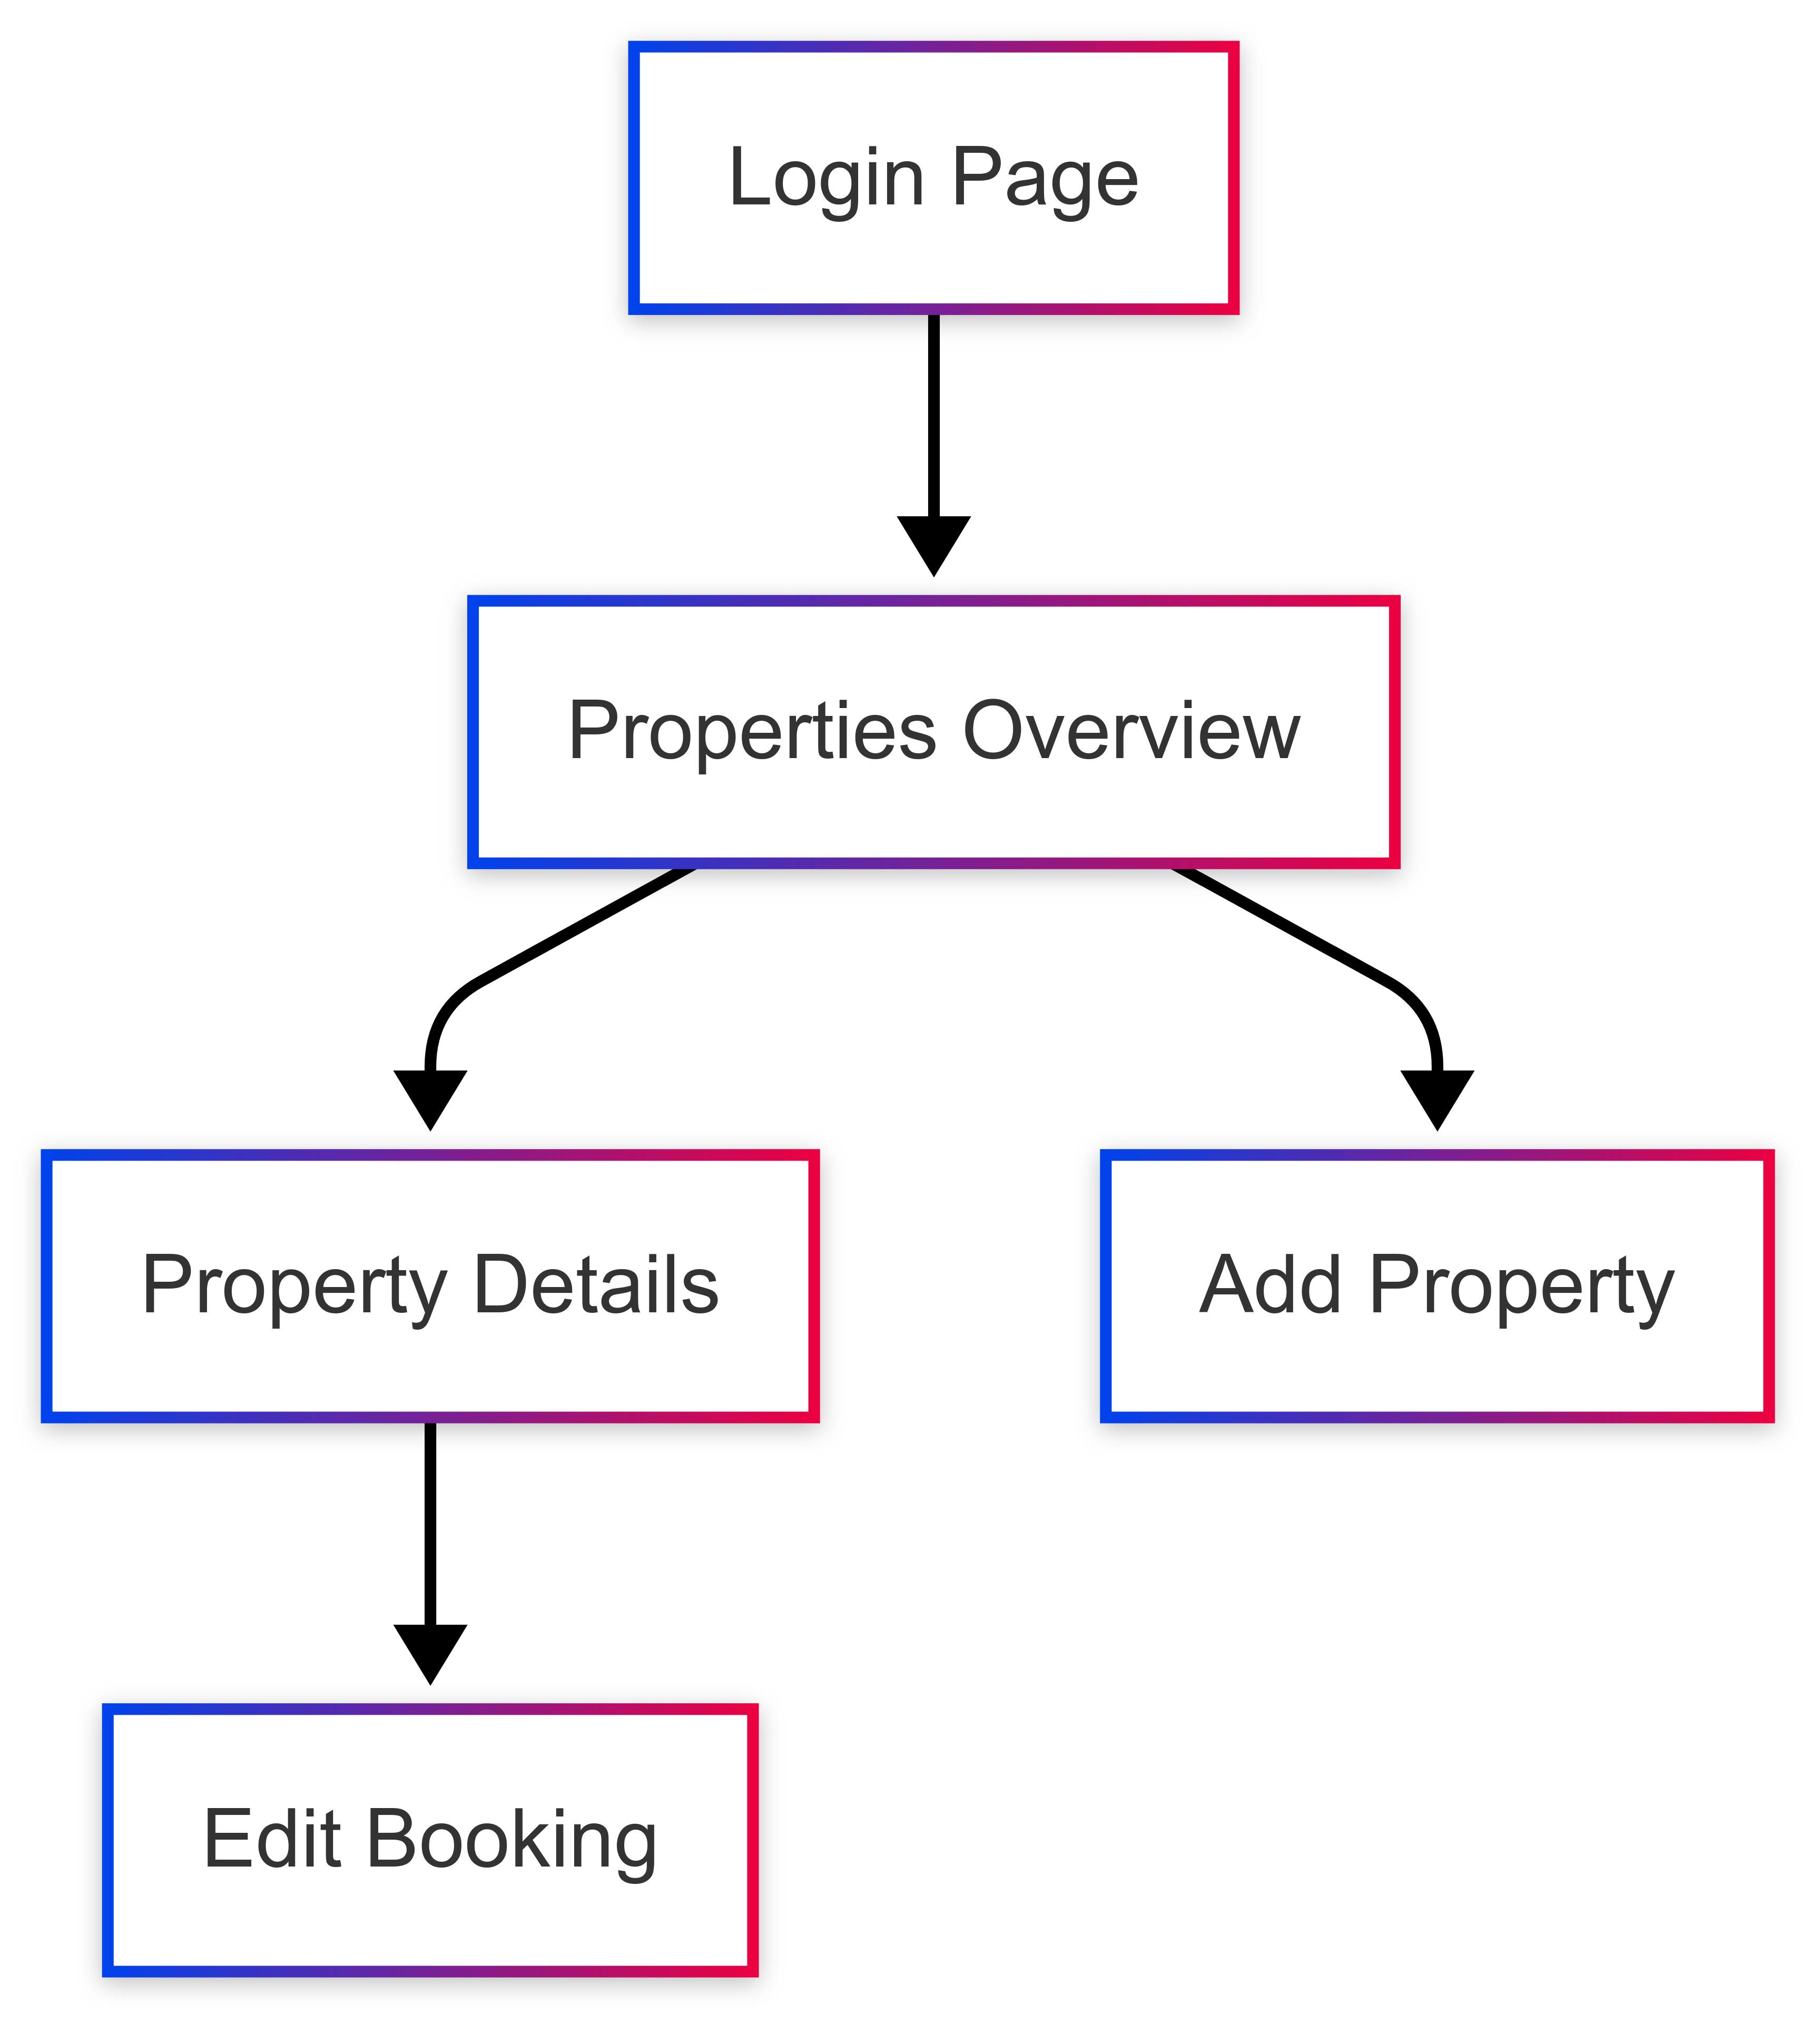
\includegraphics[width=0.55\textwidth]{images/StrukturDiagramm.png}
	\caption{Navigationsfluss der Mitarbeiteransicht}
	\label{fig:navigationsfluss}
\end{figure}

\begin{itemize}
	\item Der Einstiegspunkt ist die \textbf{Login-Seite}.
	\item Nach erfolgreichem Login gelangt man zur \textbf{Übersicht aller Immobilien} (Properties Overview).
	\item Von dort aus hat man zwei Hauptoptionen:
	\begin{itemize}
		\item \textbf{Links (Property Details)}: Details zu bestehenden Immobilien ansehen, mit der Möglichkeit, \textbf{Buchungen zu bearbeiten (Edit Booking)}.
		\item \textbf{Rechts (Add Property)}: Neue Immobilien hinzufügen.
	\end{itemize}
\end{itemize}


\subsection{Bibliotheken und Module}

\subsubsection{Importe}

Die Implementierung der Equilibria Sharing-Mitarbeiteransicht basiert auf einer Vielzahl von Bibliotheken und Modulen, die im Folgenden nach Kategorien zusammengefasst werden.
\begin{lstlisting}[language=JavaScript, caption={Kernimporte der Anwendung.}, label={listing:core-imports}]
import { redirect } from 'next/navigation'
import { useRouter } from 'next/navigation'
import { cookies } from 'next/headers'
import Image from 'next/image'
		
// Authentifizierung
import { compare } from 'bcrypt'
import { getSession } from '@/lib/session'
		
// Datenbankzugriff
import { prisma } from '@/lib/prisma'
		
// UI-Basiskomponenten
import { Button } from '@/components/ui/button'
import { Card } from '@/components/ui/card'
		
// Server-Actions
import { createProperty, updateProperty } from '@/app/actions/properties'
import { login } from '@/app/actions/auth'
\end{lstlisting}

Die in [\ref{listing:core-imports}] zusammengefassten Kernimporte repräsentieren die fundamentalen Technologien und Module, auf denen die Anwendung basiert. Next.js stellt mit \texttt{redirect}, \texttt{useRouter} und \texttt{cookies} essentielle Funktionen für Routing und Zustandsverwaltung bereit. Die Authentifizierung wird durch \texttt{bcrypt} für sichere Passwortvergleiche und die eigene \texttt{getSession}-Funktion realisiert. Der Datenbankzugriff erfolgt zentral über den \texttt{prisma}-Client, der eine sichere Interaktion mit der Datenbank ermöglicht. Für die Benutzeroberfläche werden grundlegende UI-Komponenten wie \texttt{Button} und \texttt{Card} verwendet. Die Server-Actions \texttt{login}, \texttt{createProperty} und \texttt{updateProperty} bilden das Rückgrat der serverseitigen Datenverarbeitung und gewährleisten eine sichere Handhabung sensibler Operationen.



\subsection{Authentifizierung und Sitzungsverwaltung}
\subsubsection{Login-Implementierung}
\begin{lstlisting}[language=JavaScript, caption={Benutzersuche in der Datenbank.}, label={listing:user-lookup}]
export async function login(email: string, password: string) {
	const user = await prisma.user.findUnique({
		where: { email }
	})
			
	if (!user) return { success: false, error: 'Benutzer nicht gefunden' }
\end{lstlisting}
	
	Die in [\ref{listing:user-lookup}] implementierte \texttt{login}-Funktion initiiert den Authentifizierungsprozess mit einer Datenbankabfrage. Mittels Prisma ORM wird ein Benutzer anhand seiner E-Mail-Adresse gesucht. Die frühzeitige Überprüfung auf Nichtexistenz des Benutzers stellt einen effizienten Kontrollfluss sicher und verhindert unnötige Folgeoperationen.
	
\begin{lstlisting}[language=JavaScript, caption={Passwortvalidierung und Sitzungserstellung.}, label={listing:password-validation}]
	const passwordValid = await compare(password, user.password)
			
		if (!passwordValid) return { success: false, error: 'Falsches Passwort' }
			
		const session = await createSession(user.id)
		cookies().set('session_id', session.id, { httpOnly: true })
\end{lstlisting}
	
	Der Codeabschnitt in [\ref{listing:password-validation}] realisiert zwei kritische Sicherheitsfunktionen. Zunächst erfolgt die Validierung des eingegebenen Passworts gegen den gespeicherten Hash mittels der \texttt{compare}-Funktion aus bcrypt. Bei erfolgreicher Authentifizierung wird anschließend eine neue Benutzersitzung erstellt und ein entsprechendes Cookie gesetzt. Die Verwendung des \texttt{httpOnly}-Flags verhindert dabei den Zugriff auf das Cookie via JavaScript, was einen wichtigen Schutz gegen XSS-Angriffe darstellt.
	
\begin{lstlisting}[language=JavaScript, caption={Rückgabeobjekt nach erfolgreicher Authentifizierung.}, label={listing:auth-return}]
return { 
	success: true, 
	user: { 
		id: user.id, 
		email: user.email, 
		name: user.name, 
		role: user.role 
	} 
}
\end{lstlisting}


Die Funktion schließt, wie in [\ref{listing:auth-return}] zu sehen, mit der Rückgabe eines strukturierten Objekts. Dieses signalisiert durch das \texttt{success}-Flag den erfolgreichen Abschluss des Authentifizierungsvorgangs und stellt gleichzeitig relevante Benutzerinformationen bereit. Bemerkenswert ist hierbei die bewusste Exklusion des Passwort-Hashes, was dem Prinzip der minimalen Datenweitergabe entspricht und die Sicherheit erhöht.

\subsubsection{Sitzungsverwaltung}

\begin{lstlisting}[language=JavaScript, caption={Erstellung einer neuen Sitzung.}, label={listing:session-create}]
return prisma.session.create({
	data: {
		userId,
		expiresAt: new Date(Date.now() + 30 * 24 * 60 * 60 * 1000) // 30 Tage
	}
})
\end{lstlisting}

Der in [\ref{listing:session-create}] dargestellte Funktion realisiert die Erzeugung eines neuen Sitzungseintrags in der Datenbank. Die Gültigkeitsdauer wird auf 30 Tage festgelegt, was einen angemessenen Kompromiss zwischen Benutzerkomfort und Sicherheit darstellt. Die Verknüpfung mit dem Benutzer erfolgt über die \texttt{userId}, wodurch eine eindeutige Zuordnung gewährleistet wird.

\begin{lstlisting}[language=JavaScript, caption={Abrufen einer bestehenden Sitzung.}, label={listing:session-get}]
export async function getSession() {
	const sessionId = cookies().get('session_id')?.value
		
	if (!sessionId) return null
		
	const session = await prisma.session.findUnique({
		where: { id: sessionId },
		include: { user: true }
	})
\end{lstlisting}

	
	Die Funktion \texttt{getSession()} in [\ref{listing:session-get}] bildet das Gegenstück zur Sitzungserstellung. Sie extrahiert zunächst die Sitzungs-ID aus dem Cookie-Speicher und führt eine frühzeitige Validierung durch. Diese Implementierung folgt dem Fail-Fast-Prinzip, indem sie bei fehlendem Cookie sofort abbricht und \texttt{null} zurückgibt, was die Effizienz des Codes erhöht.
	
\begin{lstlisting}[language=JavaScript, caption={Validierung der Sitzungsgültigkeit.}, label={listing:session-validate}]
if (!session || session.expiresAt < new Date()) {
	cookies().delete('session_id')
	return null
}
\end{lstlisting}


Der Codeausschnitt in [\ref{listing:session-validate}] führt eine zweistufige Validierung durch. Zunächst wird die Existenz der Sitzung in der Datenbank überprüft, gefolgt von einer Evaluation der zeitlichen Gültigkeit. Die automatische Bereinigung durch Löschen des Cookies bei ungültigen Sitzungen stellt einen proaktiven Sicherheitsmechanismus dar und verhindert potenzielle Inkonsistenzen zwischen Cookie-Zustand und Datenbankzustand.

\begin{lstlisting}[language=JavaScript, caption={Rückgabe der validierten Sitzung.}, label={listing:session-return}]
return session
\end{lstlisting}


Die in [\ref{listing:session-return}] gezeigte Rückgabe der vollständigen Sitzung inklusive der verknüpften Benutzerdaten (durch \texttt{include: \{ user: true \}}) ermöglicht einen effizienten Zugriff auf alle relevanten Informationen in einem einzigen Datenbankaufruf. Diese Optimierung reduziert die Anzahl der Datenbankabfragen und verbessert somit die Performanz der Anwendung.

\begin{lstlisting}[language=JavaScript, caption={Middleware für Routenschutz.}, label={listing:middleware-init}]
// middleware.ts
	
export function middleware(request: NextRequest) {
	const sessionId = request.cookies.get('session_id')?.value
\end{lstlisting}


Die in [\ref{listing:middleware-init}] implementierte Middleware stellt einen zentralen Baustein im Sicherheitskonzept der Anwendung dar. Sie nutzt die Next.js-Middleware-Funktionalität, um Anfragen vor dem Erreichen der eigentlichen Routen zu interceptieren. Die Extraktion der Sitzungs-ID aus den Cookies erfolgt hier direkt auf Request-Ebene, was eine effiziente Verarbeitung ermöglicht.

\begin{lstlisting}[language=JavaScript, caption={Umleitung nicht authentifizierter Anfragen.}, label={listing:middleware-redirect}]
if (!sessionId && !request.nextUrl.pathname.startsWith('/login')) {
	return NextResponse.redirect(new URL('/login', request.url))
}
		
return NextResponse.next()
}
\end{lstlisting}


Der in [\ref{listing:middleware-redirect}] dargestellte Codeblock realisiert eine automatische Umleitung nicht authentifizierter Benutzer zur Login-Seite. Die Implementierung berücksichtigt dabei intelligent den aktuellen Pfad, um Weiterleitungsschleifen zu vermeiden. Durch die Verwendung von Next.js Response-Objekten erfolgt die Umleitung serverseitig, was zusätzliche Sicherheit bietet und clientseitige Manipulationen verhindert.





\subsection{Benutzeroberfläche und Interaktionsdesign}
\subsubsection{Immobilie Übersicht}

\begin{figure}
\centering
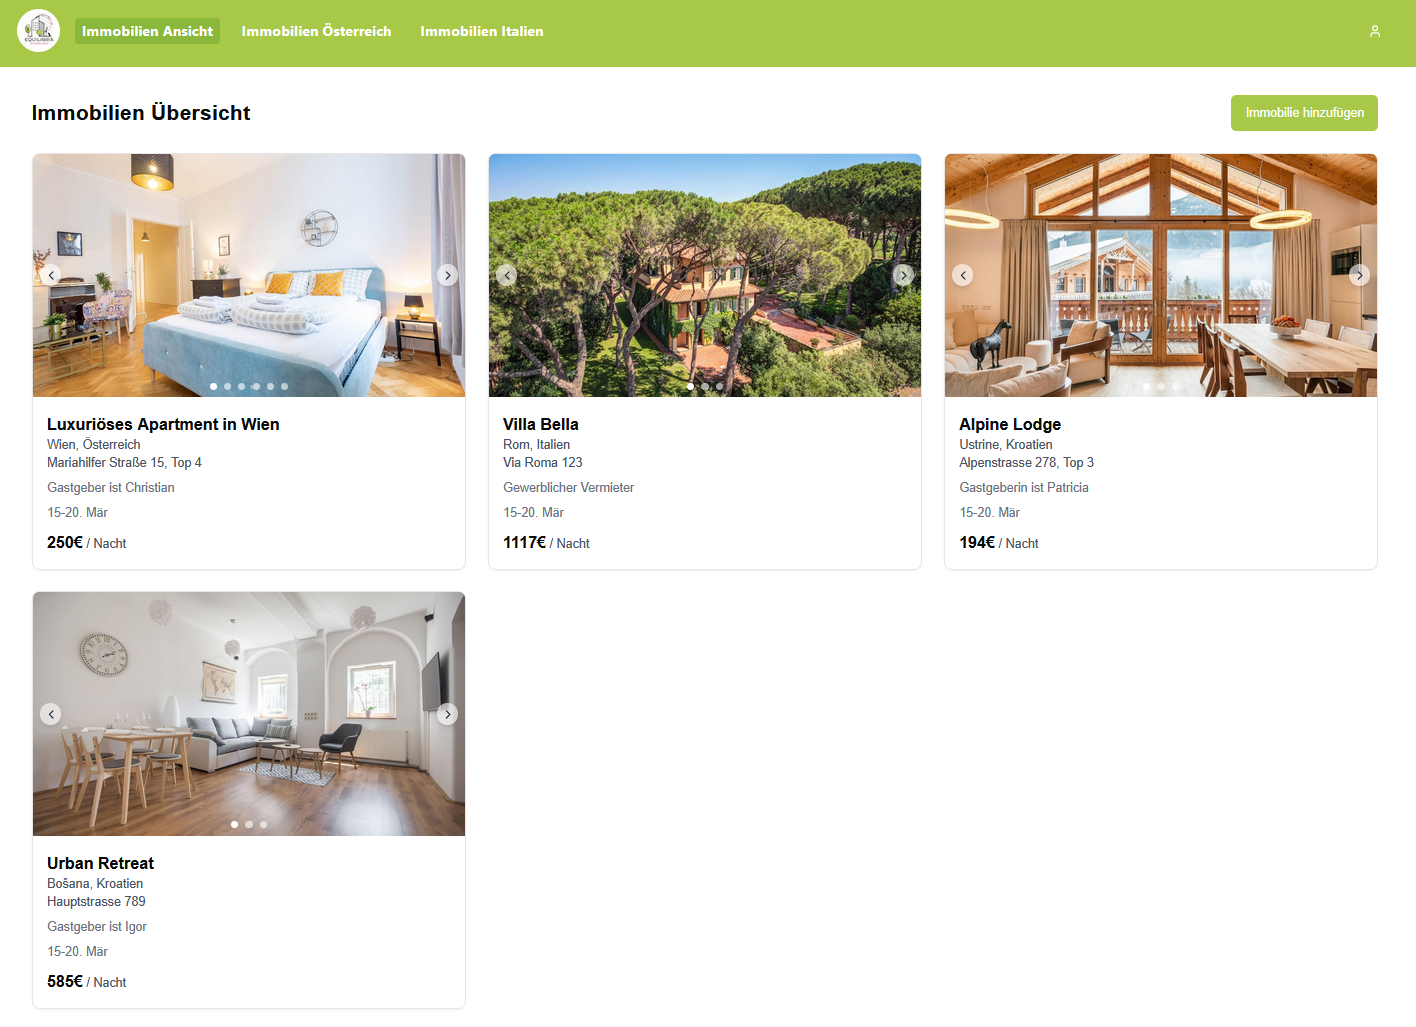
\includegraphics[width=0.80\textwidth]{images/Immobilien_Uebersicht.png}
\caption{Übersicht über alle Immobilien}
\end{figure}


\begin{lstlisting}[language=JavaScript, caption={Datenabruf für die Immobilien-Übersicht.}, label={listing:property-data-fetch}]
export default async function DashboardPage() {
	const session = await getSession()
		
	if (!session) {
		redirect('/login')
	}
		
	const properties = await prisma.property.findMany({
		where: { organizationId: session.user.organizationId },
	})
\end{lstlisting}

	
	Die Hauptkomponente in [\ref{listing:property-data-fetch}] implementiert einen serverseitigen Datenabruf. Zunächst erfolgt eine Authentifizierungsprüfung mit automatischer Weiterleitung zur Login-Seite bei fehlender Sitzung. Anschließend werden alle Immobilien der Organisation des angemeldeten Benutzers aus der Datenbank abgerufen, was eine effektive Zugriffskontrolle auf Organisationsebene realisiert.

\newpage
    
\begin{lstlisting}[language=JavaScript, caption={Header-Bereich der Übersichtsseite.}, label={listing:property-header}]
return (
<div className="container mx-auto px-4 py-8">
<div className="mb-6 flex items-center justify-between">
<h1 className="text-2xl font-bold">Immobilien Übersicht</h1>
<a href="/properties/new" className="rounded bg-primary px-4 py-2 text-white">
	Neue Immobilie
</a>
</div>
)
\end{lstlisting}

	
	Der in [\ref{listing:property-header}] implementierte Header-Bereich kombiniert einen aussagekräftigen Titel zum Hinzufügen neuer Immobilien. Die Verwendung von Tailwind CSS-Klassen ermöglicht ein responsives Layout mit konsistenten Abständen. Die semantische Struktur mit \texttt{h1} für die Hauptüberschrift verbessert zudem die Zugänglichkeit und SEO-Eigenschaften der Seite.
	
\begin{lstlisting}[language=JavaScript, caption={Rasterdarstellung der Immobilien.}, label={listing:property-grid}]
<div className="grid gap-6 md:grid-cols-2 lg:grid-cols-3">
	{properties.map((property) => (
		<PropertyCard 
		      key={property.id}
		      property={property}
		      href={`/properties/{property.id}`}
	       />
	))}
\end{lstlisting}

	
	Der in [\ref{listing:property-grid}] dargestellte Code realisiert ein responsives Raster zur Anzeige der Immobilien. Durch die Verwendung von CSS Grid mit unterschiedlichen Spaltenanzahlen je nach Bildschirmgröße wird eine optimale Darstellung auf verschiedenen Geräten gewährleistet. Die Iteration über das \texttt{properties}-Array mit der \texttt{map}-Funktion erzeugt für jede Immobilie eine \texttt{PropertyCard}-Komponente mit eindeutigem Schlüssel und Detaillink.
	
	
\begin{lstlisting}[language=JavaScript, caption={Definition der Immobilienkarten-Komponente.}, label={listing:property-card-def}]
// components/property-card.tsx

export default function PropertyCard({ property, href }) {
\end{lstlisting}

		
		Die in [\ref{listing:property-card-def}] definierte \texttt{PropertyCard}-Komponente dient der einheitlichen Darstellung von Immobilieninformationen. Die Verwendung von spezifischen Komponenten wie \texttt{Image} und \texttt{Link} optimiert die Ladezeiten und Navigation. Die importierten Icons aus der Lucide-Bibliothek ermöglichen eine intuitive visuelle Darstellung von Immobilienmerkmalen wie Standort, Schlafzimmern und Badezimmern.
		
\begin{lstlisting}[language=JavaScript, caption={Datenextraktion und Container-Struktur.}, label={listing:property-card-structure}]
const { title, price, address, bedrooms, bathrooms, area, images } = property
const imageUrl = images[0]?.url || '/placeholder.jpg'

return (
	<Link href={href} className="group overflow-hidden rounded-lg border shadow transition hover:shadow-md">
	<div className="relative h-48 w-full">
)
\end{lstlisting}

		
		Der Codeabschnitt in [\ref{listing:property-card-structure}] zeigt die Destrukturierung der Immobiliendaten und den Beginn der Kartenstruktur. Die Verwendung eines Fallback-Bildes gewährleistet eine konsistente Darstellung auch bei fehlenden Bilddaten. Der umschließende \texttt{Link} macht die gesamte Karte klickbar, während die CSS-Klassen für visuelle Effekte wie Schatten und abgerundete Ecken sorgen.
		
\begin{lstlisting}[language=JavaScript, caption={Optimierte Bilddarstellung.}, label={listing:property-image}]
<Image
	src={imageUrl || "/placeholder.svg"}
	alt={title}
	fill
	className="object-cover transition-transform group-hover:scale-105"
	sizes="(max-width: 768px) 100vw, (max-width: 1200px) 50vw, 33vw"
/>
\end{lstlisting}

		
		Die in [\ref{listing:property-image}] implementierte Bilddarstellung nutzt die \texttt{Image}-Komponente von Next.js für optimierte Ladezeiten und automatische Bildgrößenanpassung. Das \texttt{fill}-Attribut sorgt dafür, dass das Bild den Container vollständig ausfüllt, während \texttt{object-cover} ein gleichmäßiges Seitenverhältnis gewährleistet. Der Hover-Effekt mit leichter Vergrößerung (\texttt{scale-105}) bietet subtiles visuelles Feedback bei Benutzerinteraktion.
		
		
\begin{lstlisting}[language=JavaScript, caption={Darstellung der Immobilienmerkmale.}, label={listing:property-features}]
<div className="grid grid-cols-3 gap-2 text-sm">
<div className="flex items-center">
<BedDouble className="mr-1 h-4 w-4" />
<span>{bedrooms} {bedrooms === 1 ? 'Zimmer' : 'Zimmer'}</span>
</div>
<div className="flex items-center">
<Bath className="mr-1 h-4 w-4" />
\end{lstlisting}

		
		Die in [\ref{listing:property-features}] implementierte Darstellung der Immobilienmerkmale nutzt ein dreispaltiges Grid-Layout für eine übersichtliche Anordnung. Jedes Merkmal wird durch ein passendes Icon visualisiert und mit dem entsprechenden Wert kombiniert. Die bedingte Textausgabe berücksichtigt die Singular- und Pluralformen, was die sprachliche Korrektheit der Benutzeroberfläche verbessert.
		
		
		
		
		\subsubsection{Immobilie Hinzufügen}
		
		\begin{figure}
			\centering
			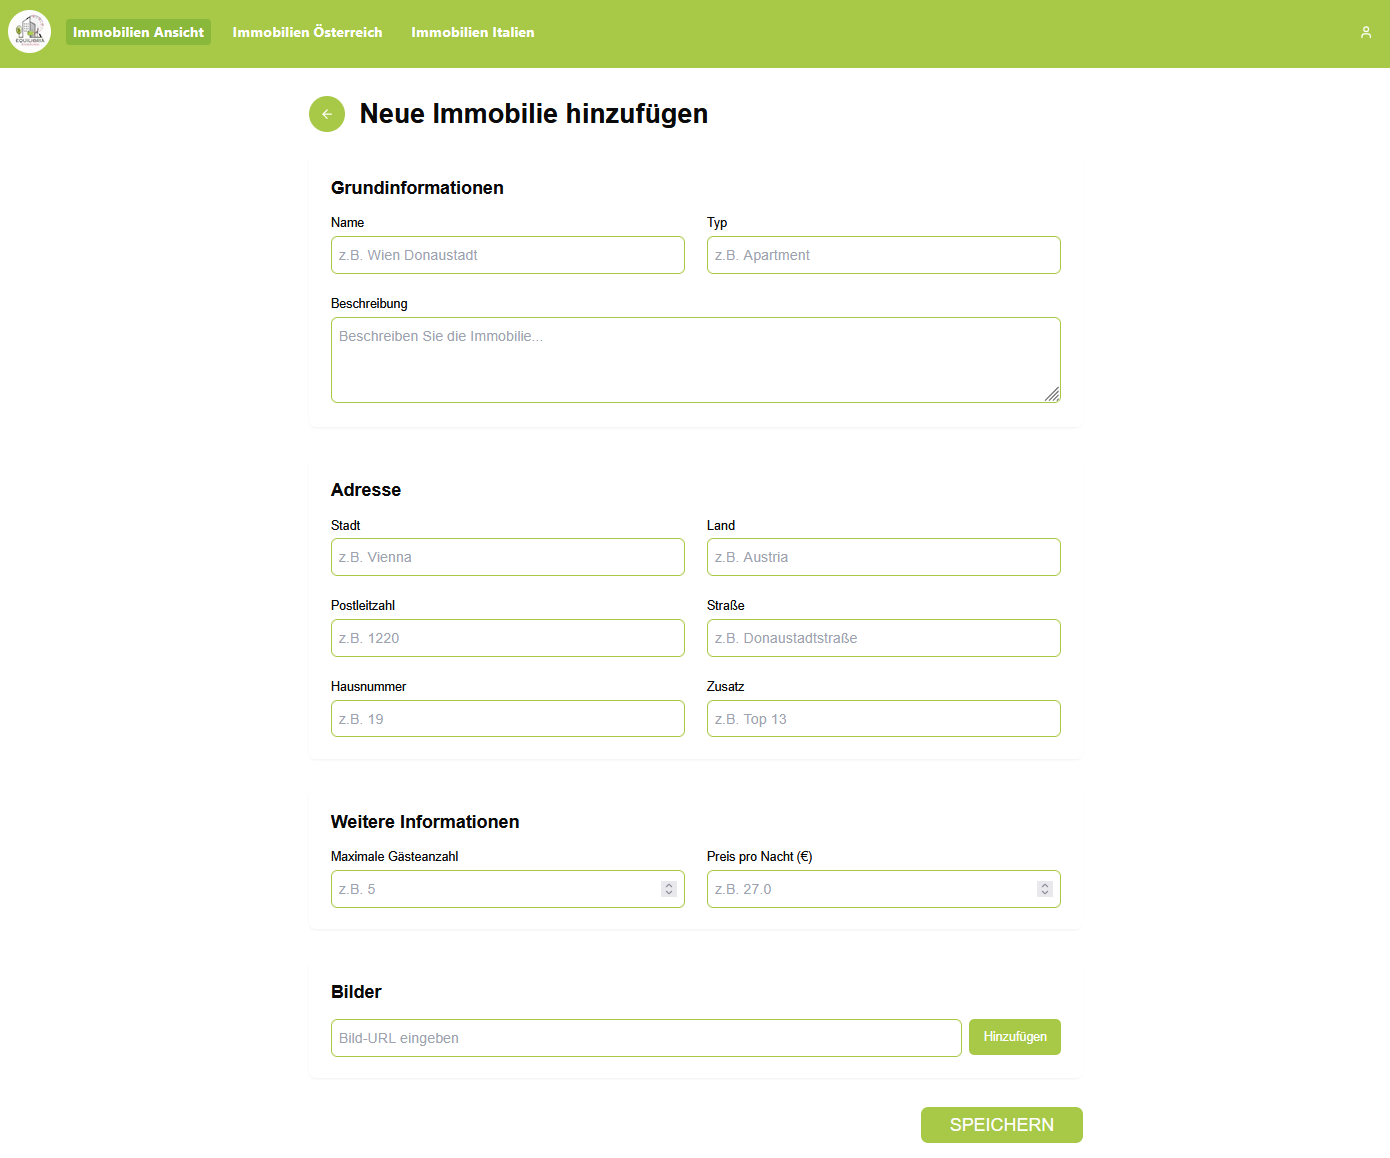
\includegraphics[width=0.80\textwidth]{images/Immobilien_hinzufuegen.png}
			\caption{Seite zum Hinzufügen von Immobilien}
		\end{figure}
		
		
\begin{lstlisting}[language=JavaScript, caption={Authentifizierungsprüfung und Container-Struktur.}, label={listing:property-add-auth}]
export default async function NewPropertyPage() {
	const session = await getSession()
					
	if (!session) {
		redirect('/login')
	}
					
	return (
	    <div className="container mx-auto px-4 py-8">
)
\end{lstlisting}

			
			Die Hauptkomponente in [\ref{listing:property-add-auth}] beginnt mit einer Authentifizierungsprüfung, die nicht angemeldete Benutzer zur Login-Seite weiterleitet. Diese Sicherheitsmaßnahme stellt sicher, dass nur autorisierte Benutzer neue Immobilien hinzufügen können. Der Container mit definierten Abständen sorgt für eine konsistente Darstellung und optimale Lesbarkeit auf verschiedenen Bildschirmgrößen.

\newpage

\begin{lstlisting}[language=JavaScript, caption={Beginn des Formularinhalts.}, label={listing:property-form-content-start}]
<form onSubmit={handleSubmit} className="space-y-6">
<div className="grid gap-6 md:grid-cols-2">
<div>
<label htmlFor="title" className="block text-sm font-medium">
Titel
</label>
\end{lstlisting}

			
			Der in [\ref{listing:property-form-content-start}] dargestellte Beginn des Formularinhalts zeigt die Verwendung eines responsiven Grid-Layouts für eine optimale Raumnutzung. Die zweispaltige Anordnung auf größeren Bildschirmen verbessert die Übersichtlichkeit und reduziert die vertikale Ausdehnung des Formulars. Die semantische Verknüpfung von Labels und Eingabefeldern durch die \texttt{htmlFor}-Attribute verbessert die Zugänglichkeit.
			
			
\begin{lstlisting}[language=JavaScript, caption={Einbindung des Immobilienformulars.}, label={listing:property-add-form}]
<PropertyForm 
	organizationId={session.user.organizationId}
	userId={session.user.id}
/>
\end{lstlisting}

		
		Die in [\ref{listing:property-add-form}] dargestellte Einbindung des Immobilienformulars übergibt wichtige Kontextinformationen aus der Benutzersitzung. Die Organisations-ID ermöglicht die korrekte Zuordnung der neuen Immobilie zur Organisation des Benutzers, während die Benutzer-ID für Audit-Zwecke und die Nachverfolgung von Änderungen verwendet wird. Diese Implementierung folgt dem Prinzip der Datensparsamkeit, indem nur die notwendigen Informationen weitergegeben werden.
		
		
\begin{lstlisting}[language=JavaScript, caption={Initialisierung der Formularkomponente.}, label={listing:property-form-init}]
export default function PropertyForm({ organizationId, userId, initialData }) {
	const router = useRouter()
	const [loading, setLoading] = useState(false)
	const [error, setError] = useState('')
					
	const [formData, setFormData] = useState(initialData || {
		title: '',
		description: '',
		price: '',
\end{lstlisting}

				
				Die Formularkomponente in [\ref{listing:property-form-init}] implementiert eine flexible Initialisierung, die sowohl für neue Immobilien als auch für die Bearbeitung bestehender Immobilien geeignet ist. Die Verwendung von \texttt{initialData} als optionaler Parameter ermöglicht die Vorausfüllung des Formulars mit existierenden Daten. Die Zustandsvariablen für Ladezustand und Fehler verbessern das Feedback während der Formularverarbeitung.
				
                
\begin{lstlisting}[language=JavaScript, caption={Behandlung von Formularänderungen.}, label={listing:property-form-change}]
const handleChange = (e) => {
	const { name, value } = e.target
				
	if (name.includes('.')) {
		const [parent, child] = name.split('.')
		setFormData({
			...formData,
			[parent]: { ...formData[parent], [child]: value }
		})
	}
}
\end{lstlisting}

						
						Die in [\ref{listing:property-form-change}] implementierte \texttt{handleChange}-Funktion ermöglicht die Aktualisierung verschachtelter Formularfelder. Durch die Analyse des Feldnamens wird erkannt, ob es sich um ein einfaches oder ein verschachteltes Feld handelt. Bei verschachtelten Feldern wie Adresskomponenten wird die entsprechende Unterstruktur im Formularstatus aktualisiert, ohne andere Werte zu beeinflussen.
						
						
\begin{lstlisting}[language=JavaScript, caption={Datenvorbereitung für die Übermittlung.}, label={listing:property-form-prepare}]
try {
	// Daten für die Übermittlung vorbereiten
	const propertyData = {
		...formData,
		price: parseFloat(formData.price),
		bedrooms: parseInt(formData.bedrooms, 10),
		bathrooms: parseInt(formData.bathrooms, 10),
		area: parseFloat(formData.area),
\end{lstlisting}

								
								Die in [\ref{listing:property-form-prepare}] dargestellte Datenvorbereitung konvertiert Zeichenkettenwerte aus dem Formular in die entsprechenden numerischen Typen. Diese Typkonvertierung ist entscheidend für die korrekte Verarbeitung in der Datenbank und verhindert potenzielle Fehler bei mathematischen Operationen oder Sortierungen. Die Verwendung von \texttt{parseFloat} und \texttt{parseInt} mit expliziter Angabe der Basis gewährleistet konsistente Ergebnisse.
\begin{lstlisting}[language=JavaScript, caption={Aufruf der Server-Action.}, label={listing:property-form-action}]
        organizationId,
        userId
    }

	// Server-Action aufrufen
	const result = await createProperty(propertyData)

	if (result.success) {
		router.push(`/properties/${result.id}`)
\end{lstlisting}

								
								Der in [\ref{listing:property-form-action}] implementierte Aufruf der Server-Action übergibt die vorbereiteten Daten an die serverseitige Funktion \texttt{createProperty}. Bei erfolgreicher Erstellung wird der Benutzer automatisch zur Detailseite der neuen Immobilie weitergeleitet.
								
\begin{lstlisting}[language=JavaScript, caption={Fehlerbehandlung bei der Formularübermittlung.}, label={listing:property-form-error}]
	router.refresh()
} else {
	setError(result.error || 'Ein Fehler ist aufgetreten')
}
} catch (err) {
	setError('Serverfehler. Bitte später erneut versuchen.')
	console.error(err)
} finally {
	setLoading(false)
}
\end{lstlisting}

					
					Die in [\ref{listing:property-form-error}] gezeigte Fehlerbehandlung fängt sowohl explizite Fehlermeldungen von der Server-Action als auch unerwartete Ausnahmen ab. Die Verwendung eines Try-Catch-Finally-Blocks gewährleistet, dass der Ladezustand in jedem Fall zurückgesetzt wird, unabhängig vom Ergebnis der Operation. Die Protokollierung von Fehlern in der Konsole erleichtert die Fehlersuche während der Entwicklung.
					
					
					
					\subsubsection{Immobilien Details}
					
					\begin{figure}
						\centering
						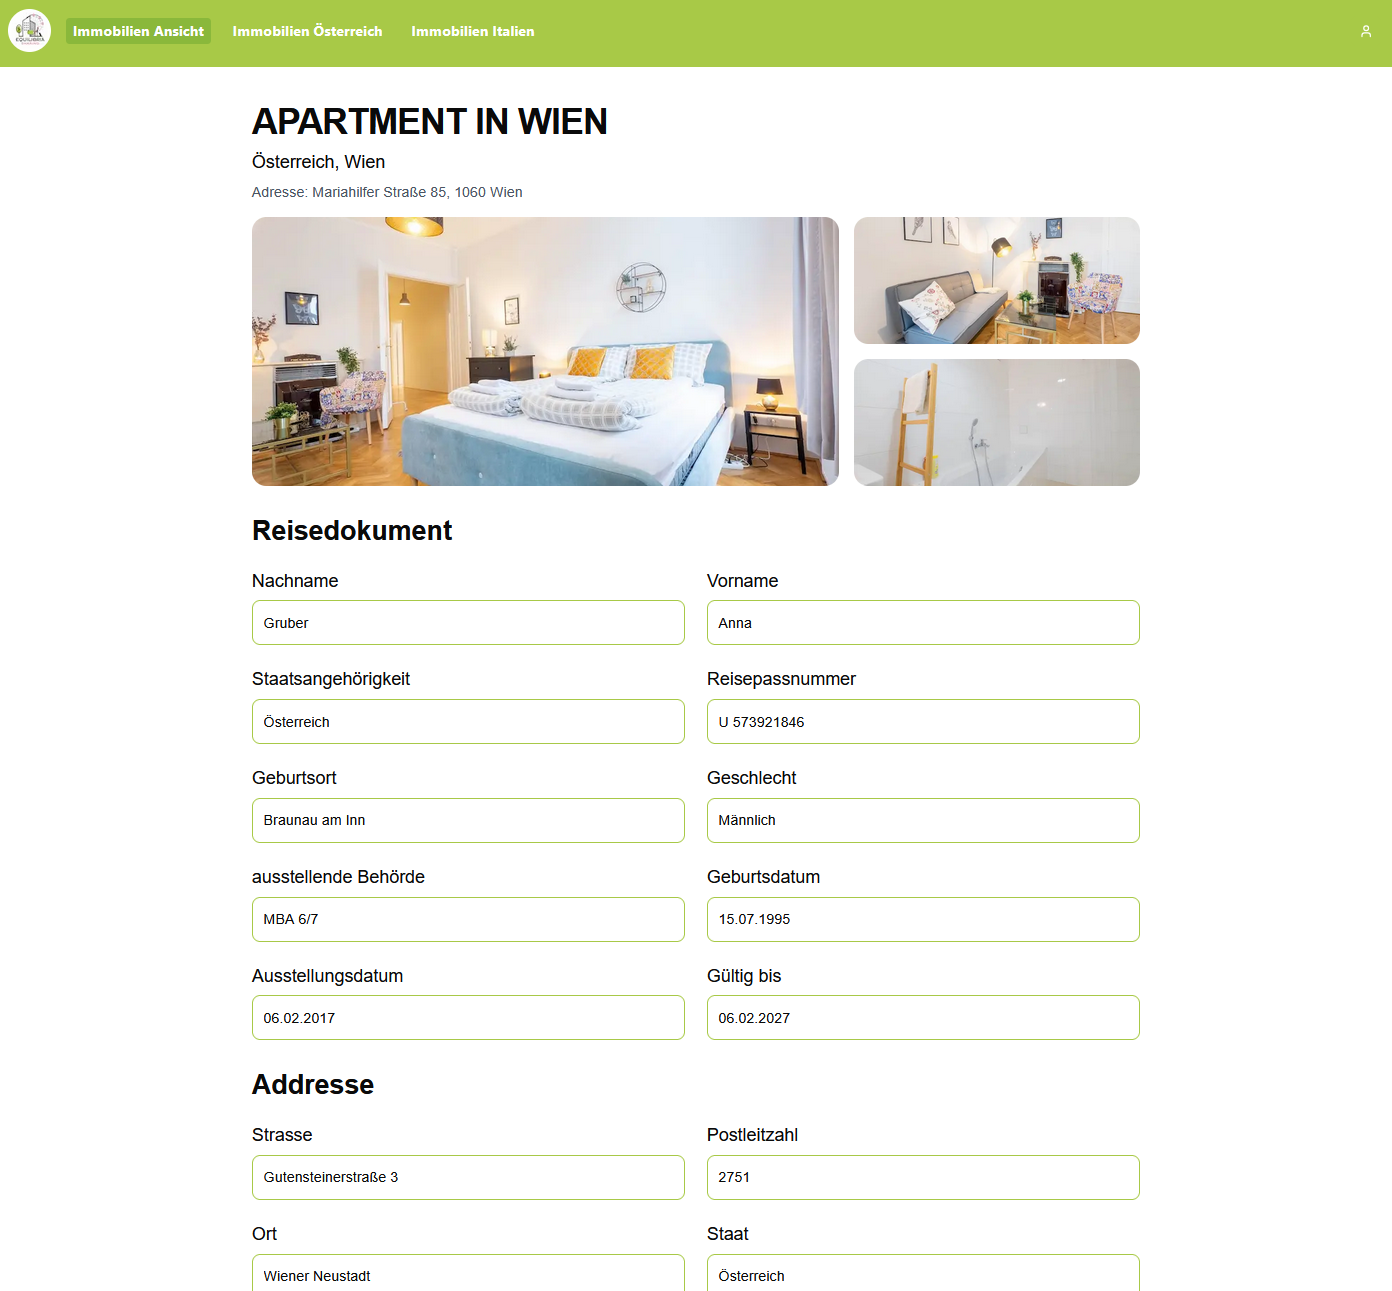
\includegraphics[width=0.80\textwidth]{images/Immobilien_bearbeiten.png}
						\caption{Buchung Bearbeitungsseite}
					\end{figure}
\begin{lstlisting}[language=JavaScript, caption={Authentifizierung und Datenabruf.}, label={listing:property-details-auth}]
export default async function PropertyPage({ params }) {
	const session = await getSession()

	if (!session) {
		redirect('/login')
	}

	const property = await prisma.property.findUnique({
		where: { id: params.id },
\end{lstlisting}

							
							Die Hauptkomponente in [\ref{listing:property-details-auth}] beginnt mit einer Authentifizierungsprüfung und leitet nicht angemeldete Benutzer zur Login-Seite weiter. Anschließend wird die spezifische Immobilie anhand der in den URL-Parametern übergebenen ID aus der Datenbank abgerufen. Diese serverseitige Datenabfrage gewährleistet, dass die Seite bereits beim ersten Laden vollständige Informationen enthält.
							
\newpage
                            
\begin{lstlisting}[language=JavaScript, caption={Zugriffskontrolle.}, label={listing:property-details-access}]
if (!property) {
	notFound()
}

// Prüfen, ob der Benutzer Zugriff auf diese Immobilie hat
if (property.organizationId !== session.user.organizationId) {
	redirect('/dashboard')
}
\end{lstlisting}

							
							Der in [\ref{listing:property-details-access}] implementierte Zugriffskontrollmechanismus stellt sicher, dass Benutzer nur auf Immobilien ihrer eigenen Organisation zugreifen können. Falls die Immobilie nicht existiert, wird die Next.js \texttt{notFound}-Funktion aufgerufen, die eine standardisierte 404-Seite rendert. Bei unberechtigtem Zugriff erfolgt eine Weiterleitung zum Dashboard, was potenzielle Sicherheitslücken durch URL-Manipulation verhindert.
							
\begin{lstlisting}[language=JavaScript, caption={Einbindung der Detailkomponente.}, label={listing:property-details-component}]
<PropertyDetails property={property} />
</div>
)
}
\end{lstlisting}

						
						Die in [\ref{listing:property-details-component}] gezeigte Einbindung der \texttt{PropertyDetails}-Komponente kapselt die eigentliche Darstellung der Immobilieninformationen. Diese Trennung von Datenabfrage und Präsentation folgt dem Prinzip der Separation of Concerns und verbessert die Wartbarkeit des Codes. Die Übergabe des vollständigen Immobilienobjekts als Prop ermöglicht eine flexible Darstellung aller verfügbaren Informationen.
						
\begin{lstlisting}[language=JavaScript, caption={Struktur der Detailkomponente.}, label={listing:property-details-structure}]
export default function PropertyDetails({ property }) {
	const { title, description, price, bedrooms, bathrooms, area, images, address, 
		createdAt, updatedAt, createdBy } = property

	return (
		<div className="grid gap-8 md:grid-cols-3">
		<div className="md:col-span-2">
\end{lstlisting}

							
							Die in [\ref{listing:property-details-structure}] implementierte Struktur der Detailkomponente verwendet ein responsives Grid-Layout, das auf größeren Bildschirmen eine asymmetrische Aufteilung mit zwei Dritteln für Hauptinhalte und einem Drittel für Zusatzinformationen bietet. Die Destrukturierung des Immobilienobjekts am Anfang der Komponente verbessert die Lesbarkeit des Codes und vereinfacht den Zugriff auf die einzelnen Eigenschaften.
\newpage
                            
\begin{lstlisting}[language=JavaScript, caption={Bilddarstellung.}, label={listing:property-details-image}]
<div className="mb-6 overflow-hidden rounded-lg">
{images && images.length > 0 ? (
    <div className="relative h-[400px] w-full">
	<Image
		src={images[0].url || "/placeholder.svg"}
	    alt={title}
	    fill
		className="object-cover"
	/>
</div>
\end{lstlisting}

								
								Die in [\ref{listing:property-details-image}] gezeigte Bilddarstellung implementiert eine bedingte Logik, die prüft, ob Bilder vorhanden sind. Das Hauptbild wird in einem Container mit fester Höhe und voller Breite dargestellt, wobei die \texttt{object-cover}-Eigenschaft ein gleichmäßiges Seitenverhältnis gewährleistet. Die Verwendung der Next.js \texttt{Image}-Komponente optimiert die Ladezeit und Bildqualität.
								
								
\begin{lstlisting}[language=JavaScript, caption={Galerie für zusätzliche Bilder.}, label={listing:property-details-gallery}]
{images && images.length > 1 && (
<div className="mb-6 grid grid-cols-4 gap-2">
{images.slice(1, 5).map((image, index) => (
<div key={image.id} className="relative h-24 overflow-hidden rounded">
<Image
	src={image.url || "/placeholder.svg"}
	alt={`${title} - Bild ${index + 2}`}
\end{lstlisting}

										
										Die in [\ref{listing:property-details-gallery}] dargestellte Bildergalerie wird nur angezeigt, wenn mehr als ein Bild vorhanden ist. Die Anordnung in einem vierspaltigen Grid ermöglicht eine kompakte Darstellung von bis zu vier zusätzlichen Bildern. Die Verwendung von \texttt{slice(1, 5)} begrenzt die Anzahl der angezeigten Vorschaubilder und verhindert eine Überladung der Benutzeroberfläche.
										
										\subsection{Zusammenfassung der Implementierung}
										
										\subsubsection{Reflexion der Herausforderungen}
										Während der Implementierung traten verschiedene Herausforderungen auf, insbesondere in den Bereichen Authentifizierung, Zustandsmanagement und API-Integration. Die korrekte Implementierung der Authentifizierung mit NextAuth.js und der Integration mit dem Backend stellte sich als komplexer heraus, als ursprünglich gedacht, da verschiedene Benutzerrollen unterschiedliche Zugriffsrechte benötigten.
										
										Ein weiteres Problem war das Fehlerhandling bei API-Anfragen. Um sicherzustellen, dass Netzwerkfehler oder Backend-Probleme nicht zu einer schlechten Benutzererfahrung führen, wurde ein zentrales Error-Handling-System entwickelt, das Fehler abfängt, protokolliert und benutzerfreundliche Fehlermeldungen anzeigt.
										
										Schließlich war die größte Herausforderung die Verwaltung des Zustandsmanagements zwischen Server- und Client-Komponenten. Denn besonders hier ist es aufgrund der unterschiedlichen Ausführungsumgebungen oft zu unerwarteten Verhaltensweisen gekommen. Die Fehlermeldungen dieser Art von Problemen waren sehr schwer zu interpretieren, da sie oft erst zur Laufzeit auftraten. Schließlich wurde eine klare Trennung zwischen Server- und Client-Komponenten geschaffen, wobei Server-Komponenten für den Datenabruf und Client-Komponenten für die interaktiven Elemente zuständig sind, was zu einer robusteren Anwendung führte.
										
										Zusätzlich zu diesen technischen Herausforderungen verzögerte sich die Frontend-Entwicklung länger als ursprünglich geplant, hauptsächlich aufgrund der Komplexität der Benutzeroberfläche und der notwendigen Anpassungen für verschiedene Endgeräte. Erschwerend kam hinzu, dass im Backend ein subtiler Fehler in der API-Schnittstelle entdeckt wurde, der die vollständige Integration zwischen Frontend und Backend verhinderte. Dieser Fehler betraf insbesondere die Datenformate bei der Übertragung von Immobilieninformationen, wodurch die Verbindung zum Backend zum Zeitpunkt der Fertigstellung noch nicht vollständig implementiert werden konnte. Stattdessen wurde für Demonstrationszwecke eine Mock-API entwickelt, die das erwartete Verhalten des Backends simuliert.
										
										
										\subsubsection{Zukünftige Erweiterungen}
										Für zukünftige Versionen sind folgende Erweiterungen denkbar:
										\begin{itemize}
											\item \textbf{Erweiterte Filterfunktionen:} Implementierung von fortschrittlicheren Suchfiltern und Sortieroptionen für Immobilien, um Mitarbeiter eine präzisere Auswahl nach spezifischen Kriterien wie zum Beispiel Ausstattungsmerkmalen zu ermöglichen.
											
											\item \textbf{Interaktive Visualisierungen:} Integration von 3D-Modellen und virtuellen Rundgängen für Immobilien, um potenziellen Interessenten einen besseren Eindruck der Objekte zu vermitteln, ohne physisch vor Ort sein zu müssen.
											
											\item \textbf{Automatisierte End-to-End-Tests:} Ausbau der Testabdeckung durch Cypress oder Playwright Tests, um kritische Benutzerflüsse wie Anmeldung, Immobiliensuche und Kontaktanfragen automatisiert zu testen und die Anwendungsstabilität zu gewährleisten.
										\end{itemize}